\chapter{Cableado Estructurado, Diseño del Rack 42U y Cómputo de Materiales}

\section{Marco Normativo Internacional Aplicable}

El diseño e implementación de la red física se rige bajo los estándares unificados de la \textbf{Telecommunications Industry Association (TIA)} y el \textbf{American National Standards Institute (ANSI)}:

\begin{enumerate}[leftmargin=*, label=\arabic*.]
    \item \textbf{ANSI/TIA-568.0-D y 568-C.2:} Establece la topología en estrella jerárquica y fija la distancia máxima del \textbf{Enlace Permanente} en \textbf{90~m}, con hasta 10~m para latiguillos, totalizando un Canal de máximo \textbf{100~m}.
    \item \textbf{ANSI/TIA-569-D:} Regula las dimensiones de canalizaciones. La ocupación inicial de cables en bandejas no debe exceder el \textbf{40\%} del área transversal, reservando el 50\% restante para crecimiento futuro.
    \item \textbf{ANSI/TIA-606-B:} Define el esquema alfanumérico para etiquetado unívoco de cables, tomas, paneles y gabinetes, garantizando la trazabilidad de cada enlace.
    \item \textbf{ANSI/TIA-607-C:} Prescribe la infraestructura de puesta a tierra equipotencial (bonding) para drenar corrientes de blindaje del cable F/UTP Cat~6A en Rayos~X y Laboratorio.
\end{enumerate}

\section{Subsistemas de Cableado Estructurado}

Al tratarse de una edificación de \textbf{un solo nivel}, no se requiere un subsistema de cableado troncal vertical entre pisos. La infraestructura se concentra en tres subsistemas operativos:

\subsection{Subsistema de Área de Trabajo (WA)}

Comprende desde la toma de pared (caja adosada con \textit{faceplate} y jacks RJ-45 Keystone hembra) hasta el equipo del usuario. Se utilizan \textbf{patch cords multifilares Cat~6 / Cat~6A de 2.0~m}, certificados de fábrica para resistir dobladuras diarias.

\subsection{Subsistema de Cableado Horizontal}

Transporta las señales desde las tomas de usuario hasta los patch panels del MDF. Emplea cable rígido monofilamento AWG~23 con forro ignífugo \textbf{LSZH}. No se permiten empalmes ni derivaciones intermedias: todos los enlaces son punto a punto directos.

\subsection{Subsistema del Cuarto de Telecomunicaciones (MDF)}

Espacio cerrado de \textbf{3.50~m $\times$ 4.20~m (14.7~m$^2$)} en el centro geográfico del edificio. Aloja el bastidor principal Rack~42U con patch panels, switches, servidores, UPS y el sistema de tierra de telecomunicaciones (TMGB).

\section{Diseño de Canalizaciones (ANSI/TIA-569-D)}

\subsection{Troncal Principal: Bandeja Tipo Malla en Pasillo Central}

\begin{itemize}[leftmargin=*]
    \item \textbf{Trayectoria:} Línea recta de 30~m suspendida a \textbf{2.75~m} en el plenum del cielo raso.
    \item \textbf{Dimensiones:} Ancho de \textbf{200~mm}, peralte de \textbf{50~mm}; acero cincado electrosoldado.
    \item \textbf{Capacidad de carga:} Área transversal útil = 10{,}000~mm$^2$. Con 56 cables Cat~6 ($\varnothing$~6.0~mm, área = 28.3~mm$^2$/cable):
    \begin{equation}
        \text{Llenado} = \frac{56 \times 28.3~\text{mm}^2}{10{,}000~\text{mm}^2} = 15.8\% \quad (\text{Límite TIA: 40\%})
    \end{equation}
\end{itemize}

\subsection{Distribución Perimetral: Canaleta de PVC de Dos Vías}

\begin{itemize}[leftmargin=*]
    \item \textbf{Especificación:} Canaleta plástica de \textbf{40~mm $\times$ 25~mm} PVC rígido autoextinguible (UL94~V-0), fijada a muros a \textbf{+0.40~m} sobre el nivel de piso terminado.
    \item \textbf{Separación de circuitos:} Tabique divisor interno continuo que aísla físicamente los cables UTP de los cables de fuerza eléctrica de 220~VAC estabilizada, mitigando la inducción electromagnética de 60~Hz.
\end{itemize}

\subsection{Puntos de Techo para Access Points}

Cuatro enlaces terminan en cajas de pase octogonales en el cielo raso a 2.60~m, con jacks hembra y latiguillos de 1.0~m para los APs PoE+ montados en el techo: AP-01 (Espera), AP-02 (Pasillo Oeste), AP-03 (Pasillo Este) y AP-04 (Administración).

\section{Estándar de Terminación T568A vs. T568B}

\subsection{Comparativa de Asignación de Pines}

\begin{table}[H]
\centering
\caption{Asignación de pines T568A vs. T568B en conector RJ-45 (8P8C)}
\small
\begin{tabularx}{\textwidth}{@{} c c c c X @{}}
\toprule
\textbf{Pin} & \textbf{Par TIA} & \textbf{T568A} & \textbf{T568B (Adoptado)} & \textbf{Función 1000BASE-T} \\
\midrule
1 & Par 3 / Par 2 & Blanco/Verde   & Blanco/Naranja & BI\_DA+ (Trx A+) \\
2 & Par 3 / Par 2 & Verde          & Naranja        & BI\_DA- (Trx A-) \\
3 & Par 2 / Par 3 & Blanco/Naranja & Blanco/Verde   & BI\_DB+ (Trx B+) \\
4 & Par 1         & Azul           & Azul           & BI\_DC+ (Trx C+) \\
5 & Par 1         & Blanco/Azul    & Blanco/Azul    & BI\_DC- (Trx C-) \\
6 & Par 2 / Par 3 & Naranja        & Verde          & BI\_DB- (Trx B-) \\
7 & Par 4         & Blanco/Marrón  & Blanco/Marrón  & BI\_DD+ (Trx D+) \\
8 & Par 4         & Marrón         & Marrón         & BI\_DD- (Trx D-) \\
\bottomrule
\end{tabularx}
\label{tab:t568b}
\end{table}

\begin{figure}[H]
\centering
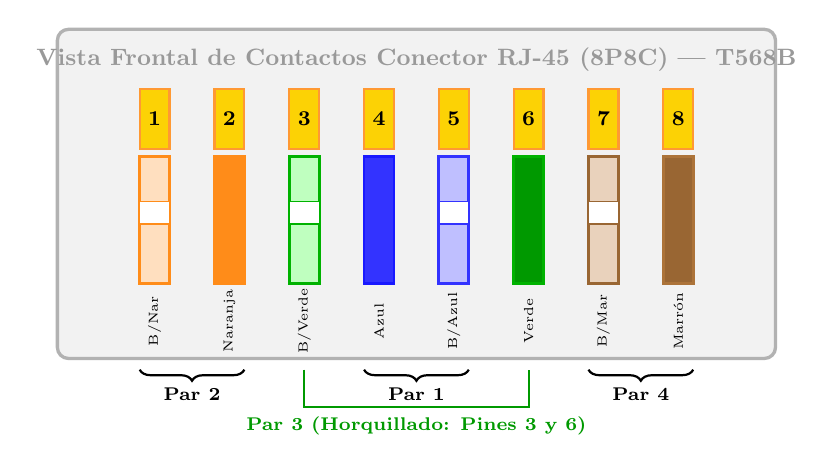
\begin{tikzpicture}[scale=0.95, every node/.style={transform shape}]
    % Contorno del conector RJ-45
    \draw[fill=gray!10, draw=gray!60, rounded corners=4pt, line width=1.2pt] (-0.8, -0.6) rectangle (8.8, 3.8);
    \node[font=\bfseries\small, text=gray!80] at (4, 3.4) {Vista Frontal de Contactos Conector RJ-45 (8P8C) --- T568B};

    % Cuchillas / Pines dorados
    \foreach \i in {1,...,8} {
        \draw[fill=yellow!70!orange, draw=orange!80, line width=0.8pt] (\i-0.7, 2.2) rectangle (\i-0.3, 3.0);
        \node[font=\bfseries\footnotesize] at (\i-0.5, 2.6) {\i};
    }

    % Conductores de colores T568B
    % 1: Blanco/Naranja
    \draw[fill=orange!25, draw=orange!90, line width=1pt] (0.3, 0.4) rectangle (0.7, 2.1);
    \draw[fill=white, draw=orange!90, line width=0.5pt] (0.3, 1.2) rectangle (0.7, 1.5);
    \node[font=\tiny, align=center, rotate=90] at (0.5, -0.1) {B/Nar};

    % 2: Naranja
    \draw[fill=orange!90, draw=orange!90, line width=1pt] (1.3, 0.4) rectangle (1.7, 2.1);
    \node[font=\tiny, align=center, rotate=90] at (1.5, -0.1) {Naranja};

    % 3: Blanco/Verde
    \draw[fill=green!25, draw=green!70!black, line width=1pt] (2.3, 0.4) rectangle (2.7, 2.1);
    \draw[fill=white, draw=green!70!black, line width=0.5pt] (2.3, 1.2) rectangle (2.7, 1.5);
    \node[font=\tiny, align=center, rotate=90] at (2.5, -0.1) {B/Verde};

    % 4: Azul
    \draw[fill=blue!80, draw=blue!90, line width=1pt] (3.3, 0.4) rectangle (3.7, 2.1);
    \node[font=\tiny, align=center, rotate=90, text=white] at (3.5, 1.25) {};
    \node[font=\tiny, align=center, rotate=90] at (3.5, -0.1) {Azul};

    % 5: Blanco/Azul
    \draw[fill=blue!25, draw=blue!80, line width=1pt] (4.3, 0.4) rectangle (4.7, 2.1);
    \draw[fill=white, draw=blue!80, line width=0.5pt] (4.3, 1.2) rectangle (4.7, 1.5);
    \node[font=\tiny, align=center, rotate=90] at (4.5, -0.1) {B/Azul};

    % 6: Verde
    \draw[fill=green!60!black, draw=green!70!black, line width=1pt] (5.3, 0.4) rectangle (5.7, 2.1);
    \node[font=\tiny, align=center, rotate=90] at (5.5, -0.1) {Verde};

    % 7: Blanco/Marrón
    \draw[fill=brown!35, draw=brown!80!black, line width=1pt] (6.3, 0.4) rectangle (6.7, 2.1);
    \draw[fill=white, draw=brown!80!black, line width=0.5pt] (6.3, 1.2) rectangle (6.7, 1.5);
    \node[font=\tiny, align=center, rotate=90] at (6.5, -0.1) {B/Mar};

    % 8: Marrón
    \draw[fill=brown!80!black, draw=brown!90!black, line width=1pt] (7.3, 0.4) rectangle (7.7, 2.1);
    \node[font=\tiny, align=center, rotate=90] at (7.5, -0.1) {Marrón};

    % Agrupación por pares TIA
    \draw[decorate, decoration={brace, amplitude=4pt, mirror}, line width=0.8pt] (0.3,-0.75) -- (1.7,-0.75) node[midway, below=3pt, font=\scriptsize\bfseries] {Par 2};
    \draw[decorate, decoration={brace, amplitude=4pt, mirror}, line width=0.8pt] (3.3,-0.75) -- (4.7,-0.75) node[midway, below=3pt, font=\scriptsize\bfseries] {Par 1};
    \draw[decorate, decoration={brace, amplitude=4pt, mirror}, line width=0.8pt] (6.3,-0.75) -- (7.7,-0.75) node[midway, below=3pt, font=\scriptsize\bfseries] {Par 4};
    \draw[line width=0.8pt, green!60!black] (2.5, -0.75) -- (2.5, -1.25) -- (5.5, -1.25) -- (5.5, -0.75);
    \node[font=\scriptsize\bfseries, green!60!black] at (4.0, -1.5) {Par 3 (Horquillado: Pines 3 y 6)};
\end{tikzpicture}
\caption{Diagrama esquemático de terminación normalizada T568B en conector RJ-45 (8P8C)}
\label{fig:t568b}
\end{figure}

\subsection{Justificación de la Elección de T568B}

\begin{enumerate}[leftmargin=*, label=\arabic*.]
    \item \textbf{Estándar de facto en Perú y Latinoamérica:} La totalidad de los patch cords comerciales y periféricos preexistentes vienen con terminación T568B.
    \item \textbf{Consistencia de enlace:} Todos los jacks Keystone, patch panels y latiguillos del policlínico están ponchados bajo T568B en ambos extremos, conformando un \textbf{cable directo (\textit{straight-through})} certificado.
\end{enumerate}

\section{Diseño del Gabinete Rack 42U (MDF)}

Se implementa un \textbf{Gabinete de Telecomunicaciones cerrado de 42U} (19'', 800~mm de profundidad, puerta de vidrio templado con cerradura). La distribución vertical optimiza la separación térmica y la ergonomía de parcheo:

\begin{figure}[H]
\centering
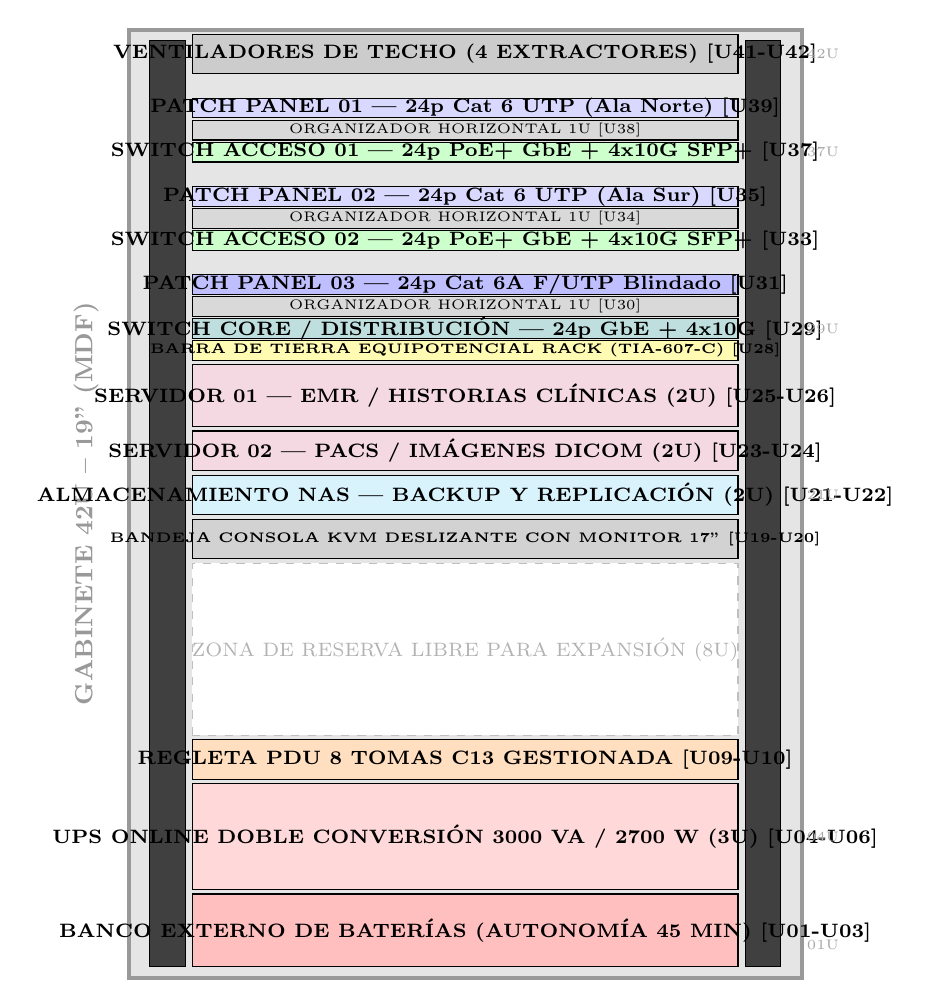
\begin{tikzpicture}[xscale=0.9, yscale=0.28]
    % Perfil exterior del Rack 42U
    \draw[fill=gray!20, draw=gray!80, line width=1.5pt] (0,0) rectangle (9.5, 43);
    \node[font=\bfseries\small, text=gray!80, rotate=90] at (-0.6, 21.5) {GABINETE 42U -- 19'' (MDF)};

    % Guías de rack izquierda y derecha
    \draw[fill=black!75] (0.3, 0.5) rectangle (0.8, 42.5);
    \draw[fill=black!75] (8.7, 0.5) rectangle (9.2, 42.5);

    % Módulos internos
    % U41-U42: Ventilación
    \draw[fill=gray!40, draw=black] (0.9, 41) rectangle (8.6, 42.8);
    \node[font=\scriptsize\bfseries] at (4.75, 41.9) {VENTILADORES DE TECHO (4 EXTRACTORES) [U41-U42]};

    % U39: Patch Panel 01
    \draw[fill=blue!15, draw=black] (0.9, 39) rectangle (8.6, 39.9);
    \node[font=\scriptsize\bfseries] at (4.75, 39.45) {PATCH PANEL 01 --- 24p Cat 6 UTP (Ala Norte) [U39]};

    % U38: Organizador 01
    \draw[fill=gray!30, draw=black] (0.9, 38) rectangle (8.6, 38.9);
    \node[font=\tiny] at (4.75, 38.45) {ORGANIZADOR HORIZONTAL 1U [U38]};

    % U37: Switch Acceso 01
    \draw[fill=green!20, draw=black] (0.9, 37) rectangle (8.6, 37.9);
    \node[font=\scriptsize\bfseries] at (4.75, 37.45) {SWITCH ACCESO 01 --- 24p PoE+ GbE + 4x10G SFP+ [U37]};

    % U35: Patch Panel 02
    \draw[fill=blue!15, draw=black] (0.9, 35) rectangle (8.6, 35.9);
    \node[font=\scriptsize\bfseries] at (4.75, 35.45) {PATCH PANEL 02 --- 24p Cat 6 UTP (Ala Sur) [U35]};

    % U34: Organizador 02
    \draw[fill=gray!30, draw=black] (0.9, 34) rectangle (8.6, 34.9);
    \node[font=\tiny] at (4.75, 34.45) {ORGANIZADOR HORIZONTAL 1U [U34]};

    % U33: Switch Acceso 02
    \draw[fill=green!20, draw=black] (0.9, 33) rectangle (8.6, 33.9);
    \node[font=\scriptsize\bfseries] at (4.75, 33.45) {SWITCH ACCESO 02 --- 24p PoE+ GbE + 4x10G SFP+ [U33]};

    % U31: Patch Panel 03
    \draw[fill=blue!25, draw=black] (0.9, 31) rectangle (8.6, 31.9);
    \node[font=\scriptsize\bfseries] at (4.75, 31.45) {PATCH PANEL 03 --- 24p Cat 6A F/UTP Blindado [U31]};

    % U30: Organizador 03
    \draw[fill=gray!30, draw=black] (0.9, 30) rectangle (8.6, 30.9);
    \node[font=\tiny] at (4.75, 30.45) {ORGANIZADOR HORIZONTAL 1U [U30]};

    % U29: Switch Core
    \draw[fill=teal!25, draw=black] (0.9, 29) rectangle (8.6, 29.9);
    \node[font=\scriptsize\bfseries] at (4.75, 29.45) {SWITCH CORE / DISTRIBUCIÓN --- 24p GbE + 4x10G [U29]};

    % U28: Tierra F/UTP
    \draw[fill=yellow!30, draw=black] (0.9, 28) rectangle (8.6, 28.9);
    \node[font=\tiny\bfseries] at (4.75, 28.45) {BARRA DE TIERRA EQUIPOTENCIAL RACK (TIA-607-C) [U28]};

    % U25-U27: Servidor HCE
    \draw[fill=purple!15, draw=black] (0.9, 25) rectangle (8.6, 27.8);
    \node[font=\scriptsize\bfseries] at (4.75, 26.4) {SERVIDOR 01 --- EMR / HISTORIAS CLÍNICAS (2U) [U25-U26]};

    % U23-U24: Servidor PACS
    \draw[fill=purple!15, draw=black] (0.9, 23) rectangle (8.6, 24.8);
    \node[font=\scriptsize\bfseries] at (4.75, 23.9) {SERVIDOR 02 --- PACS / IMÁGENES DICOM (2U) [U23-U24]};

    % U21-U22: NAS
    \draw[fill=cyan!15, draw=black] (0.9, 21) rectangle (8.6, 22.8);
    \node[font=\scriptsize\bfseries] at (4.75, 21.9) {ALMACENAMIENTO NAS --- BACKUP Y REPLICACIÓN (2U) [U21-U22]};

    % U19-U20: KVM Console
    \draw[fill=gray!35, draw=black] (0.9, 19) rectangle (8.6, 20.8);
    \node[font=\tiny\bfseries] at (4.75, 19.9) {BANDEJA CONSOLA KVM DESLIZANTE CON MONITOR 17'' [U19-U20]};

    % U11-U18: Reserva de Expansión
    \draw[fill=white, draw=gray!50, dashed] (0.9, 11) rectangle (8.6, 18.8);
    \node[font=\scriptsize, text=gray!60] at (4.75, 14.9) {ZONA DE RESERVA LIBRE PARA EXPANSIÓN (8U)};

    % U09-U10: PDU
    \draw[fill=orange!25, draw=black] (0.9, 9) rectangle (8.6, 10.8);
    \node[font=\scriptsize\bfseries] at (4.75, 9.9) {REGLETA PDU 8 TOMAS C13 GESTIONADA [U09-U10]};

    % U04-U08: UPS Online
    \draw[fill=red!15, draw=black] (0.9, 4) rectangle (8.6, 8.8);
    \node[font=\scriptsize\bfseries] at (4.75, 6.4) {UPS ONLINE DOBLE CONVERSIÓN 3000~VA / 2700~W (3U) [U04-U06]};

    % U01-U03: Baterías
    \draw[fill=red!25, draw=black] (0.9, 0.5) rectangle (8.6, 3.8);
    \node[font=\scriptsize\bfseries] at (4.75, 2.15) {BANCO EXTERNO DE BATERÍAS (AUTONOMÍA 45 MIN) [U01-U03]};

    % Cotas de altura U
    \node[font=\tiny, text=gray!70] at (9.8, 41.9) {42U};
    \node[font=\tiny, text=gray!70] at (9.8, 37.45) {37U};
    \node[font=\tiny, text=gray!70] at (9.8, 29.45) {29U};
    \node[font=\tiny, text=gray!70] at (9.8, 21.9) {21U};
    \node[font=\tiny, text=gray!70] at (9.8, 6.4) {04U};
    \node[font=\tiny, text=gray!70] at (9.8, 1.5) {01U};
\end{tikzpicture}
\caption{Elevación frontal y distribución vertical del Gabinete Rack 42U del MDF}
\label{fig:rack42u}
\end{figure}

\begin{table}[H]
\centering
\caption{Distribución vertical del Gabinete Rack 42U --- Vista frontal}
\small
\begin{tabularx}{\textwidth}{@{} c >{\raggedright\arraybackslash}p{3.8cm} X @{}}
\toprule
\textbf{U\#} & \textbf{Elemento} & \textbf{Descripción Técnica} \\
\midrule
U41--U42 & Ventilación    & Bandeja de 4 extractores de techo con termostato \\
U40      & Reserva        & Espacio libre para expansión futura \\
U39      & Patch Panel 01 & 24 puertos Cat~6 UTP --- Puestos 01 al 24 (Ala Norte) \\
U38      & Organizador 1U & Ducto ranurado de doble anillo para patch cords \\
U37      & Switch Acceso 01 & 24p Gigabit PoE+ Layer~2 (370~W) + 4 uplinks SFP+~10G \\
U36      & Libre 1U       & Espacio de ventilación entre switches \\
U35      & Patch Panel 02 & 24 puertos Cat~6 UTP --- Puestos 25 al 48 (Ala Sur) \\
U34      & Organizador 1U & Ducto ranurado de doble anillo \\
U33      & Switch Acceso 02 & 24p Gigabit PoE+ Layer~2 (370~W) + 4 uplinks SFP+~10G \\
U32      & Libre 1U       & Espacio de ventilación \\
U31      & Patch Panel 03 & 24 puertos Cat~6A F/UTP Blindado --- Puestos 49--56 + reservas \\
U30      & Organizador 1U & Ducto ranurado de doble anillo \\
U29      & Switch Core    & 24p GbE + 4 puertos SFP+~10G (distribución/núcleo) \\
U28      & Tierra F/UTP   & Barra de aterrizado para blindaje Cat~6A (TIA-607-C) \\
U25--U27 & Servidor 01    & Historias Clínicas Electrónicas (HCE/EMR) --- 2U \\
U23--U24 & Servidor 02    & PACS --- Archivo Digital de Imágenes DICOM --- 2U \\
U21--U22 & NAS            & Almacenamiento de respaldo y copias de seguridad --- 2U \\
U19--U20 & KVM            & Bandeja deslizante monitor/teclado de servicio \\
U11--U18 & Expansión      & 8U libres para servidores futuros \\
U09--U10 & PDU            & Regleta PDU horizontal 8 tomas C13 con interruptor térmico \\
U04--U08 & UPS Online     & Doble conversión 3000~VA / 2700~W --- 3U \\
U01--U03 & Baterías       & Banco externo para UPS (autonomía 45~min) --- 3U \\
\bottomrule
\end{tabularx}
\label{tab:rack}
\end{table}

\section{Cómputo Métrico de Cable y Bill of Materials}

\subsection{Metodología de Cálculo}

Se aplica la siguiente fórmula estándar de ingeniería, con un factor de seguridad del 10\% para senos de dilatación, radios de curvatura y remates de conectorización:

\begin{equation}
L_{\text{enlace}} = \bigl(d_{\text{horizontal}} + d_{\text{bajada techo}} + d_{\text{bajada rack}}\bigr) \times 1.10
\end{equation}

Las bajadas verticales fijas suman: $2.20~\text{m}$ (cielo raso a toma de pared) $+ 2.00~\text{m}$ (bandeja a base de parcheo en rack) $= \mathbf{4.20~\text{m por enlace}}$.

\subsection{Cable UTP Categoría 6 (50 Puntos)}

\begin{equation}
\text{Metros UTP Cat~6} = 50~\text{puntos} \times \bigl(16.50 + 4.20\bigr)~\text{m} \times 1.10 = \mathbf{1{,}138.5~\text{m}}
\end{equation}
\begin{equation}
\text{Bobinas} = \frac{1{,}138.5~\text{m}}{305~\text{m}} = 3.73 \longrightarrow \mathbf{4~\text{bobinas de 305~m}} \quad (\text{remanente: }81.5~\text{m})
\end{equation}

\subsection{Cable F/UTP Categoría 6A Blindado (6 Puntos)}

\begin{equation}
\text{Metros F/UTP Cat~6A} = 6~\text{puntos} \times \bigl(18.00 + 4.20\bigr)~\text{m} \times 1.10 = \mathbf{146.5~\text{m}}
\end{equation}
\begin{equation}
\text{Bobinas} = \frac{146.5~\text{m}}{305~\text{m}} = 0.48 \longrightarrow \mathbf{1~\text{bobina de 305~m}}
\end{equation}

\subsection{Resumen del Bill of Materials (BOM)}

\begin{table}[H]
\centering
\caption{Bill of Materials --- Resumen de componentes principales}
\small
\begin{tabularx}{\textwidth}{@{}clXcc@{}}
\toprule
\textbf{Ítem} & \textbf{Código} & \textbf{Descripción} & \textbf{Cant.} & \textbf{Unidad} \\
\midrule
01 & CAB-CAT6   & Bobina UTP Cat~6 LSZH 23~AWG (305~m)               & 4  & Rollo \\
02 & CAB-CAT6A  & Bobina F/UTP Cat~6A Blindado LSZH 23~AWG (305~m)   & 1  & Rollo \\
03 & JK-CAT6    & Jack Keystone RJ-45 Cat~6 UTP hembra               & 50 & Pza   \\
04 & JK-CAT6A   & Jack Keystone RJ-45 Cat~6A Blindado metálico        & 6  & Pza   \\
05 & FP-2V      & Faceplate termoplástico 2 ventanas                  & 23 & Pza   \\
06 & FP-4V      & Faceplate termoplástico 4 ventanas                  & 2  & Pza   \\
07 & PC-UTP-2M  & Patch Cord UTP Cat~6 LSZH 2.0~m                    & 46 & Pza   \\
08 & PC-UTP-1M  & Patch Cord UTP Cat~6 LSZH 1.0~m (rack)             & 50 & Pza   \\
09 & PC-FTP-2M  & Patch Cord F/UTP Cat~6A Blindado 2.0~m             & 6  & Pza   \\
10 & PC-FTP-1M  & Patch Cord F/UTP Cat~6A Blindado 1.0~m (rack)      & 6  & Pza   \\
11 & PP-24-C6   & Patch Panel 24p Cat~6 UTP 19''~1U                  & 2  & Pza   \\
12 & PP-24-C6A  & Patch Panel 24p Cat~6A Blindado con tierra          & 1  & Pza   \\
13 & ORG-1U     & Organizador horizontal 1U 19'' doble anillo         & 3  & Pza   \\
14 & RCK-42U    & Gabinete Rack 42U 19'', profundidad 800~mm          & 1  & Pza   \\
15 & UPS-3KVA   & UPS Online Doble Conversión 3000~VA / 2700~W        & 1  & Pza   \\
16 & SW-ACC-POE & Switch L2 Administrable 24p GbE PoE+ + 4 SFP+~10G  & 2  & Pza   \\
17 & SW-CORE    & Switch Distribución 24p GbE + 4 SFP+~10G           & 1  & Pza   \\
18 & AP-WIFI6   & Access Point Wi-Fi~6 (802.11ax) Dual Band PoE+     & 4  & Pza   \\
\bottomrule
\end{tabularx}
\label{tab:bom}
\end{table}
